\chapter{Pitch Excited Coding (LPC) and Vocal Tract Models}
\label{ch:part4}

Pitch Excied codeing af LPC går du på at skældne mellem frames og bestemme om de er ''voiced'' eller ''unnvoiced'' hvilket betyder om framen indeholder relative lave frekvenser som i udtalte vil være nasale eller høje frekvenser som kan betegnes som sshhhh lyde..
Fordelen ved denne methode er, at de unvoiced frames kan erstattes med gaussisk hvid støj i decoder enden og derved kan data transmitionen reduceres. Selektionen mellem voiced og unvoiced frames udføres ved at se på autokorralationen af signalet. Hvis vi Fx. ser på en frame på 20ms, hvis det lokale maksimum mellem 3ms til 15 ms oversiger 25$\%$ af energien til tid 0 (=r[0]) er der tale om en voiced frame. Hvis den derimod er under de 25$\%$ er det en unvoiced frame.

  Hvis vi kaster opmærksomheden på (a) og (b) som er udvalgte frames fra den udleveret ''oak'' audio filen. Vi har brugt matlab filen SpeechLPC.m til analysen hvor frame længten er på 20ms og overlappet er på 10ms. på figur \ref{fig:part4_autoko}  
kan vi se at den første frame (a) er voiced og at frame(b) er unvoiced da det højeste punkt mellem 3ms og 15ms ikke oversiger 25$\%$ af energien i tid 0. 

 \begin{figure}[!h]
	\centering
	\subfloat[Voiced]{%
		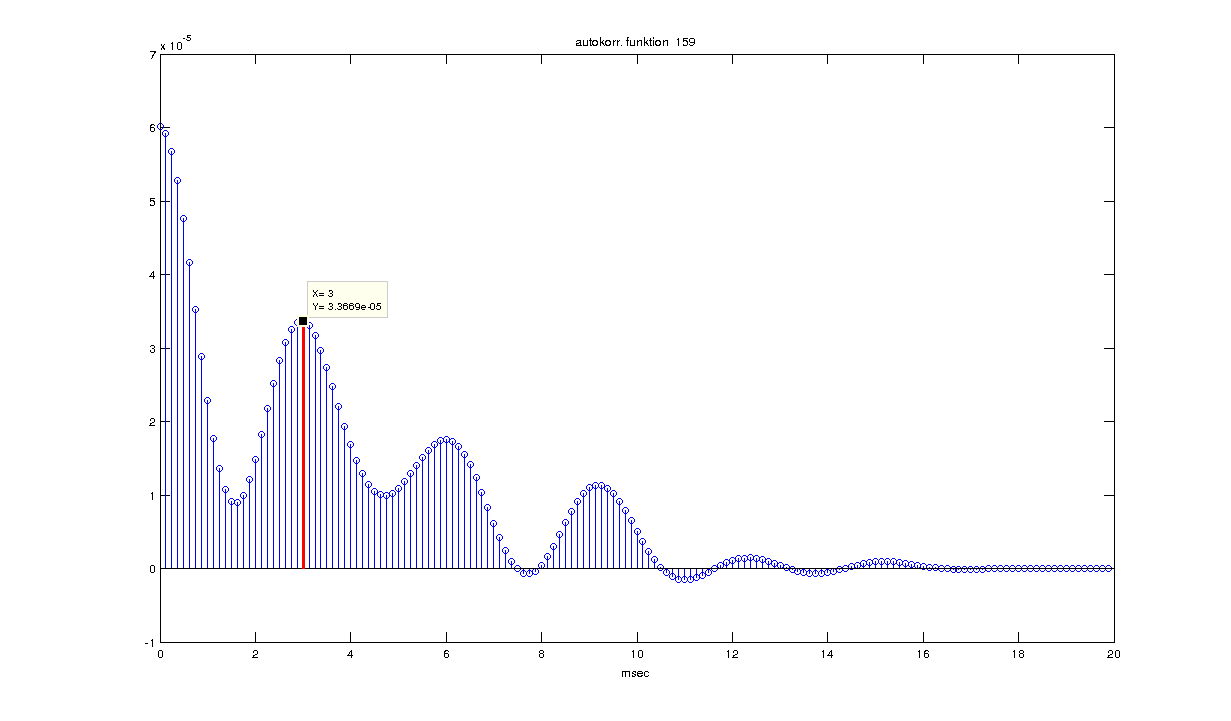
\includegraphics[width=0.5\textwidth]{resources/part4_voiced_autoko.png}
		\label{fig:part4_1}}
	\subfloat[unvoiced]{%
		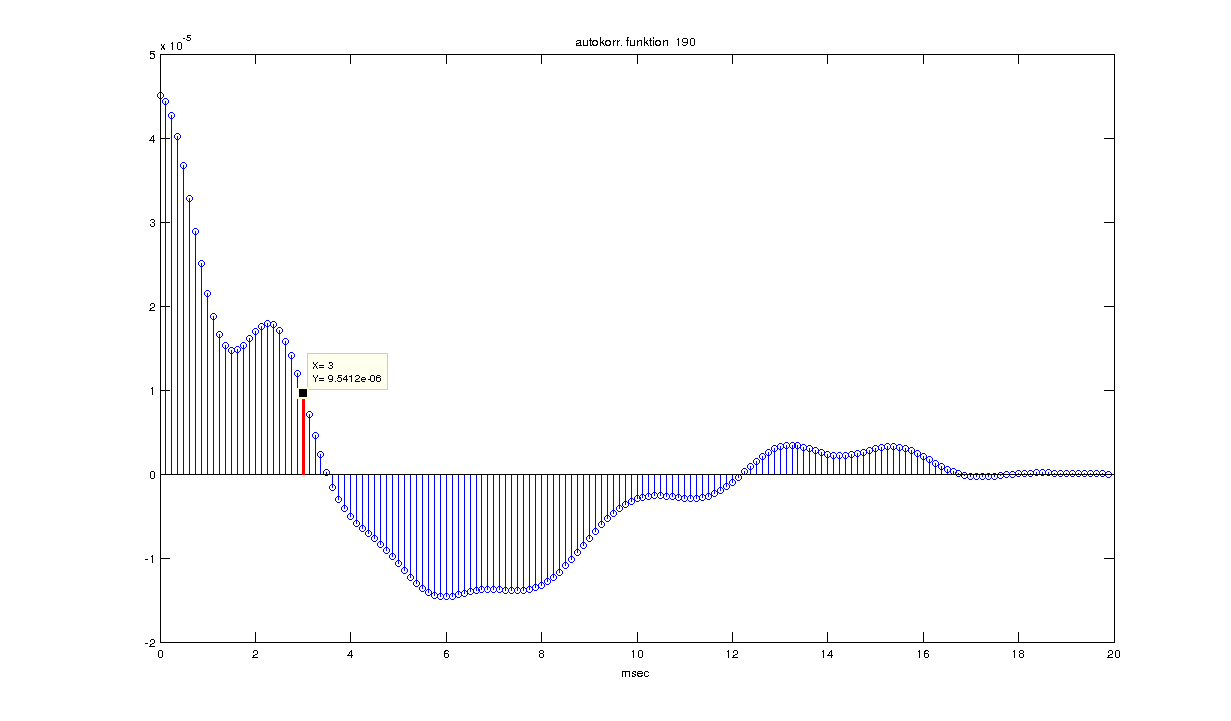
\includegraphics[width=0.5\textwidth]{resources/part4_unvoiced_autoko.png}
		\label{fig:part4_2}}
	\caption{ Autokorraltion af frame 159 og frame 190}
	\label{fig:part4_autoko}
\end{figure}

For at verificere dette resultat ser vi på frekvensresponsen for framen (a) og frame (b):
 \begin{figure}[!h]
	\centering
	\subfloat[Voiced]{%
		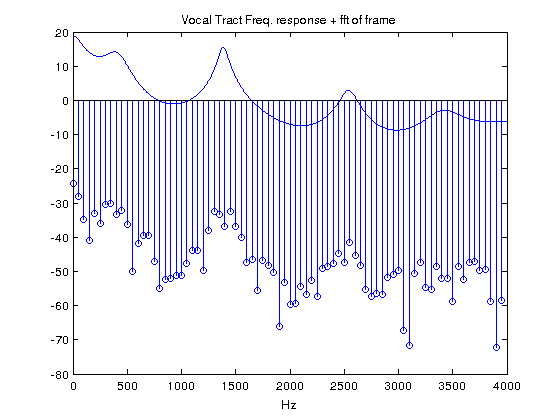
\includegraphics[width=0.5\textwidth]{resources/part4_voiced_vocaltrack.png}
		\label{fig:part4_3}}
	\subfloat[unvoiced]{%
		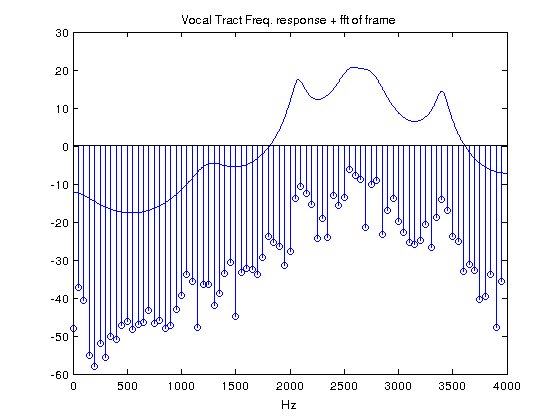
\includegraphics[width=0.5\textwidth]{resources/part4_unvoiced_vocaltrack.png}
		\label{fig:part4_4}}
	\caption{ Frekvensrespons og fft af frame 159 og frame 190 }
	\label{fig:part4_vocaltrack}
\end{figure}

Her se vi ganske rigtigt af frekvensresponset af frame(a) indeholder ''lave'' frekvenser hvor frekvensresponset af frame(b) har flere ''høje'' frekvenser komponenter.
Af udlemperne ved denne methode kan nævnes at kvaliteten af det genskabte signal er forholdsvis lav. Den gaussiske hvide støj gengiver  unvoiced frame med kun et udtryk hvor den naturlige tale har mange gengivelser af dette frekvens område.   